\documentclass{beamer}

\usepackage{graphics}
\usepackage{graphicx}
\usepackage{amsmath,amssymb,amsthm}
%\usepackage{subeqnarray}
%\usepackage{easybmat}
%\usepackage{subfigure}



%\usepackage{HA-prosper}
%\usepackage[dvips,letterpaper]{geometry}


\def\R{\mathbb{R}}
\def\Rzero{\mathcal{R}_0}
\def\diag{\textrm{diag}}
\def\tr{\textrm{tr}}
\def\det{\textrm{det}}
\def\sgn{\textrm{sgn}}
\def\imply{$\Rightarrow$}

\begin{document}
\maketitle

%%%%%%%%%%%%%%
%%%%%%%%%%%%%

\frame{\frametitle{Cell division}
\begin{block}{Definition}
Cell division is the process by which a cell, called the parent cell, divides into two cells, called daughter cells. Cell division is usually a small segment of a larger cell cycle.
\begin{itemize}
\item Prokaryotic cells: binary fission
\item Eukaryotic cells: mitosis+cytokinesis
\end{itemize}
\end{block}
}


\frame{\frametitle{Binary fission}
{\footnotesize The prokaryotic chromosome is a single DNA molecule that first replicates, then attaches each copy to a different part of the cell membrane. When the cell begins to pull apart, the replicate and original chromosomes are separated. Following cell splitting (cytokinesis), there are then two cells of identical genetic composition (except for the rare chance of a spontaneous mutation).}
\begin{center}
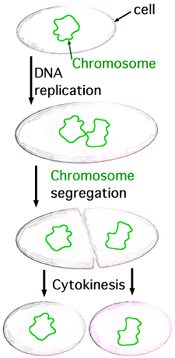
\includegraphics[width=.25\textwidth]{Binary_fission}
\end{center}
}



\frame{\frametitle{Mitosis+Citokinesis}
Mitosis is the process by which a cell separates its duplicated genome into two identical halves. It is generally followed immediately by cytokinesis which divides the cytoplasm and cell membrane. This results in two identical daughter cells with a roughly equal distribution of organelles and other cellular components. Mitosis and cytokinesis together is defined as the mitotic (M) phase of the cell cycle, the division of the mother cell into two daughter cells, each the genetic equivalent of the parent cell.
\begin{center}
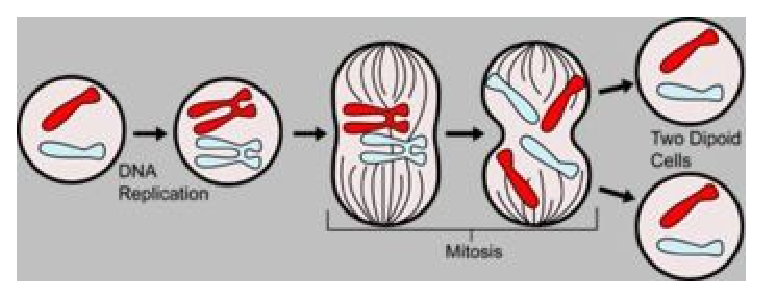
\includegraphics[width=.8\textwidth]{Mitosis}
\end{center}
}


\frame{
\begin{block}{Example 1}
E. coli are able to divide every 20 minutes under optimal conditions. Describe the temporal evolution of a colony of E. coli.
\end{block}

\begin{block}{Example 2}
Assume that adult females of a species produce offspring at a fixed period of time each year. A proportion of the offspring (juveniles) survives to adulhood, reproduces, and dies (nonoverlapping of generations). Let
\begin{itemize}
\item $j_t$ number of juveniles in years $t$
\item $a_t$ number of adult females in year $t$
\item $p$ number of juveniles that survive in year $t$
\item $f$ number of offspring produced per female
\item $r$ ratio of females to adults.
\end{itemize}
\end{block}}


\frame{
\begin{block}{Example 3}
A drug is administred once every four hours. Let $D_n$ be the amount of the drug in the blood system at the $n^{th}$ interval.  The body eliminates a certain fraction $p$ of the drug during each time interval. If the amount administred is $D_0$, find $D_n$ and $\lim _{n \rightarrow}D_{n}$.
\end{block}



\begin{block}{Example 4}
Plants produce seeds at the end of their growth season (August), after which they die. A fraction of these seeds survive the winter, and some of these germinate at the beginning of the season (May), giving rise to the new generation of plants. The fraction that germinates depends on the age of the seeds. 

Additional assumption: Seeds older than two years are no longer viable

\begin{itemize}
\item $\gamma$ number of seeds produced per plant in August
\item $\sigma$ fraction of seeds that survive a given winter
\item $\alpha$ fraction of one-year-old seeds that germinate in May
\item $\beta$ fraction of two-year-old seeds that germinate in May
\end{itemize}
\end{block}


}


%\begin{block}{Example 2b}
%Now assume that juveniles (offspring) do not become reproductive adults until their second years, and all adults do not die.
%\begin{itemize}
%\item $p_a$ fraction of female adults that survive each year.
%\end{itemize}
%\end{block}



%\frame{\frametitle{Difference equations}
%\begin{itemize}
%
%\item changes of states are descibed over discrete intervals.
%\item length of the discrete interval is some fixed length $\Delta t$: states of a system are modeled at the discrete time $t=0,\Delta t, 2\Delta t, \dots$
%\item Notation: time interval is often simplified $\Delta t=1$, and the state of the system at time $t$ as $x_t$
%\item to describe populations whose generations do not overlap.
%\end{itemize}
%
%}


\frame{\frametitle{Difference equations}
\begin{block}{Definition}
A difference equation of order $k$ has the form $$f(x_{t+k},x_{t+k-1},\dots,x_{t+1},x_t,t)=0\quad t=0,1,\dots,$$
where $f$ is a real-valued function of the real variable $x_t$ through $x_{t+k}$ and $t$.
\end{block}
\begin{block}{Order }
The order of a difference equation is the difference between the largest and the smallest arguments $k$ appearing in it.
\end{block}
\begin{block}{Autonomous - Nonautonomous}
The difference equation is called autonomous if $f$ does not depend explicitly on $t$ and it is called nonautonomous otherwise.
\end{block}
}



\frame{\frametitle{Difference equations}
$$x_{t+k}+a_1 x_{t+k-1}+a_2 x_{t+k-2}+\dots +a_{k-1} x_{t+1}=b_t \quad t=0,1,\dots$$

\begin{block}{Linear - Nonlinear}
If the coefficients $a_j$, $j=1,\dots , k$ are constant or depend on $t$ but {\bf do not depend on the state variables}, then the difference equation is said to be {linear}; otherwise, it is to be nonlinear. 
\end{block}

\begin{block}{Homogeneous - Nonhomogeneous}
If the difference equation is linear and $b_t=0$ for all $t$, then it is said to be homogeneous; otherwise, it is said to be nonhomogeneous.
\end{block}

}



\frame{\frametitle{Solution of difference equation}
\begin{block}{Definition}
A solution of the difference equation
$$f(x_{t+k},x_{t+k-1},\dots,x_{t+1},x_t,t)=0\quad t=0,1,\dots,$$
is a function $x_t$, $t=0,1,2,\dots$ such that when substituted into the equation makes it a true statement.
\end{block}

}


\frame{\frametitle{First-order linear homogeneous difference equation}
$$x_{t+1}=ax_t$$
If $x_0$ (initial value) is known, the solution is unique and is
$$x_t=a^tx_0$$
\begin{itemize}
\item $0<a<1$ then $\lim_{t\rightarrow \infty}x_t=0$
\item $a=1$ then $x_t=x_0$ $\forall t$
\item $a>1$ then $\lim_{t\rightarrow \infty}x_t=+\infty$
\end{itemize}


In general
\begin{itemize}
\item $|a|<1$ $x_t$ converges to 0.
\item $a=1$ $x_t$ is constant.
\item $|a|>1$ $x_t$ diverges (either approaches infinity or oscillates).
\end{itemize}

}


\frame{\frametitle{First-order linear homogeneous difference equation}
$$x_{t+1}=a(t)x_t \quad t=0,1,2,\dots$$
If $x_0$ (initial value) is known, the solution is unique and is
$$x_t=\left [\prod_{i=0}^{t-1} a(i)\right ]x_0$$

}


\frame{\frametitle{First-order linear nonhomogeneous difference equation}
$$x_{t+1}=a(t)x_t + b(t)\quad t=0,1,2,\dots$$
If $x_0$ (initial value) is known, the solution is unique and is
$$x_t=\left [\prod_{i=0}^{t-1} a(i)\right ]x_0 +b(t-1)+\sum_{i=0}^{t-2}\left [ \prod_{r=i+1}^{t-1} a(r) \right]b(i)$$
\begin{block}{}
\begin{itemize}
\item $x_{t+1}=a x_t + b(t)\quad x(0)=x_0$, then $$x_t=a ^t x_0 +\sum_{i=0}^{t-1} a^{t-i-1}b(i)$$
\item $x_{t+1}=a x_t + b \quad x(0)=x_0$, then 
$$x_t=\left \{ \begin{array}{ll}a ^t x_0 +b\left[\frac{a^t-1}{a-1}\right] & a\not =1\\  x_0 +bt & a =1
\end{array}
\right.$$
\end{itemize}
\end{block}

}

%\frame{\frametitle{Second-order and higher order linear homogeneous equations with constant coefficients}
%An $m^{th}-$order equation
%$$a_0x_{t+m}+a_1x_{t+m-1}+\dots + a_m x_{t}=0$$
%the order $m$ of the equation is the number of previous generations that directly influence the value of $x$ in a given generation.
%
%Solutions are composed of linear combinations of expressions of the form
%$$x_t=C\lambda ^t$$
%where $\lambda$ are obtained by finding the roots of the characteristic equation, that are called the eigenvalues.
%$$a_0\lambda^{m}+a_1\lambda^{m-1}+\dots + a_m =0$$
%
%The form of the solutions depends on the eigenvalues and there exist 3 cases:
%\begin{itemize}
%\item Eigenvalues are real and distinct: $\lambda _1 \not = \lambda 2 \dots \not = \lambda _m$. The the $m$ linearly independent solutions are  $x_t^1=\lambda _1^t$, $\dots$, $x_t^m=\lambda _m^t$. The general solution is
%$$x_t=c_1\lambda _1 ^t+\dots+c_m\lambda _m ^t$$
%\end{itemize}
%
%}


%\frame{\frametitle{Graphical method: Cobwebbing}}

\end{document}
